% !TEX root = ../om_ts_002.tex

\begin{frame} % название фрагмента

\videotitle{ARIMA process}

\end{frame}



\begin{frame}{ARIMA process: Plan}
  \begin{itemize}[<+->]
	\item Stationarity of $ARMA$
	\item Definition of $ARIMA$
	\item Differencing
  \end{itemize}

\end{frame}



\begin{frame}
	\frametitle{Nuances}
	
	\begin{itemize}
		\onslide<1->{\item Process $y_t \sim ARMA(p, q)$ is stationary \alert{by definition}:}
		
		\onslide<2->{$\E(y_t) = \mu_y$, $\Var(y_t) = \gamma_0$, $\Cov(y_t, y_{t-k}) = \gamma_k$}
		
		\onslide<3->{\item In the \alert{canonical notation} $ARMA(p, q)$ of the process $P(L) y_t = c+ Q(L) u_t$ for the polynomial $P(L)$
			all roots $\abs{\ell} > 1$}
				
		\onslide<4->{\item When estimating the $ARMA(p, q)$ process by the maximum likelihood method, these restrictions are imposed \alert{a priori}}
		
	\end{itemize}
	
\end{frame}


\begin{frame}
	\frametitle{What to do with non-stationary processes?}
	
	\begin{block}{Definition}
		The random process $(y_t)$ is called the $ARIMA(p, 1, q)$ w.r.t. the white noise process $(u_t)$,
		if $(y_t)$ is non-stationary, but $\Delta y_t$ is a stationary $ARMA(p, q)$ process w.r.t. the  white noise $(u_t)$
	\end{block}
	
	\pause
	
	\begin{block}{Definition}
		The random process $(y_t)$ is called the $ARIMA(p, 2, q)$ w.r.t. the  white noise process $(u_t)$,
		if $(y_t)$ and $(\Delta y_t)$ are non-stationary, but $\Delta^2 y_t$ is a stationary $ARMA(p, q)$ process w.r.t. the white noise $(u_t)$
	\end{block}
	
	\pause
	$\Delta y_t = y_t - y_{t-1}$ and $\Delta^2 y_t = \Delta y_t - \Delta y_{t-1}$
	
	\pause
	ARIMA — \alert{A}uto\alert{R}egressive \alert{I}ntegrated \alert{M}oving \alert{A}verage
	
\end{frame}

\begin{frame}
	\frametitle{How to choose?}
	
	$ARIMA(p, 0, q)$ or $ARIMA(p, 1, q)$ or $ARIMA(p, 2, q)$
	\begin{itemize}
		\onslide<2->{\item Analyse the \alert{graph}:}
		\onslide<3->{stationary process graph oscillates around its mean with a \alert{constant deviation}}
		
		\onslide<4->{\item Evaluate all the models and choose the best one by \alert{cross-validation}}
		\onslide<5->{Time consuming!}
		
		\onslide<6->{\item \alert{You cannot use $AIC$}!}
		
		\onslide<7->{$\ln L(y_1, \ldots, y_n \mid \theta)$ and $\ln L(y_2, \ldots, y_n \mid \theta, y_1)$ and $\ln L( y_3, \ldots, y_n \mid \theta, y_1, y_2)$
			incomparable!}
		\onslide<8->{\item There are \alert{unit root tests}!}
		
		\onslide<9->{ADF, KPSS, PP, \ldots}
	\end{itemize}
	
\end{frame}

\begin{frame}
	\frametitle{Analysing the graphs}
	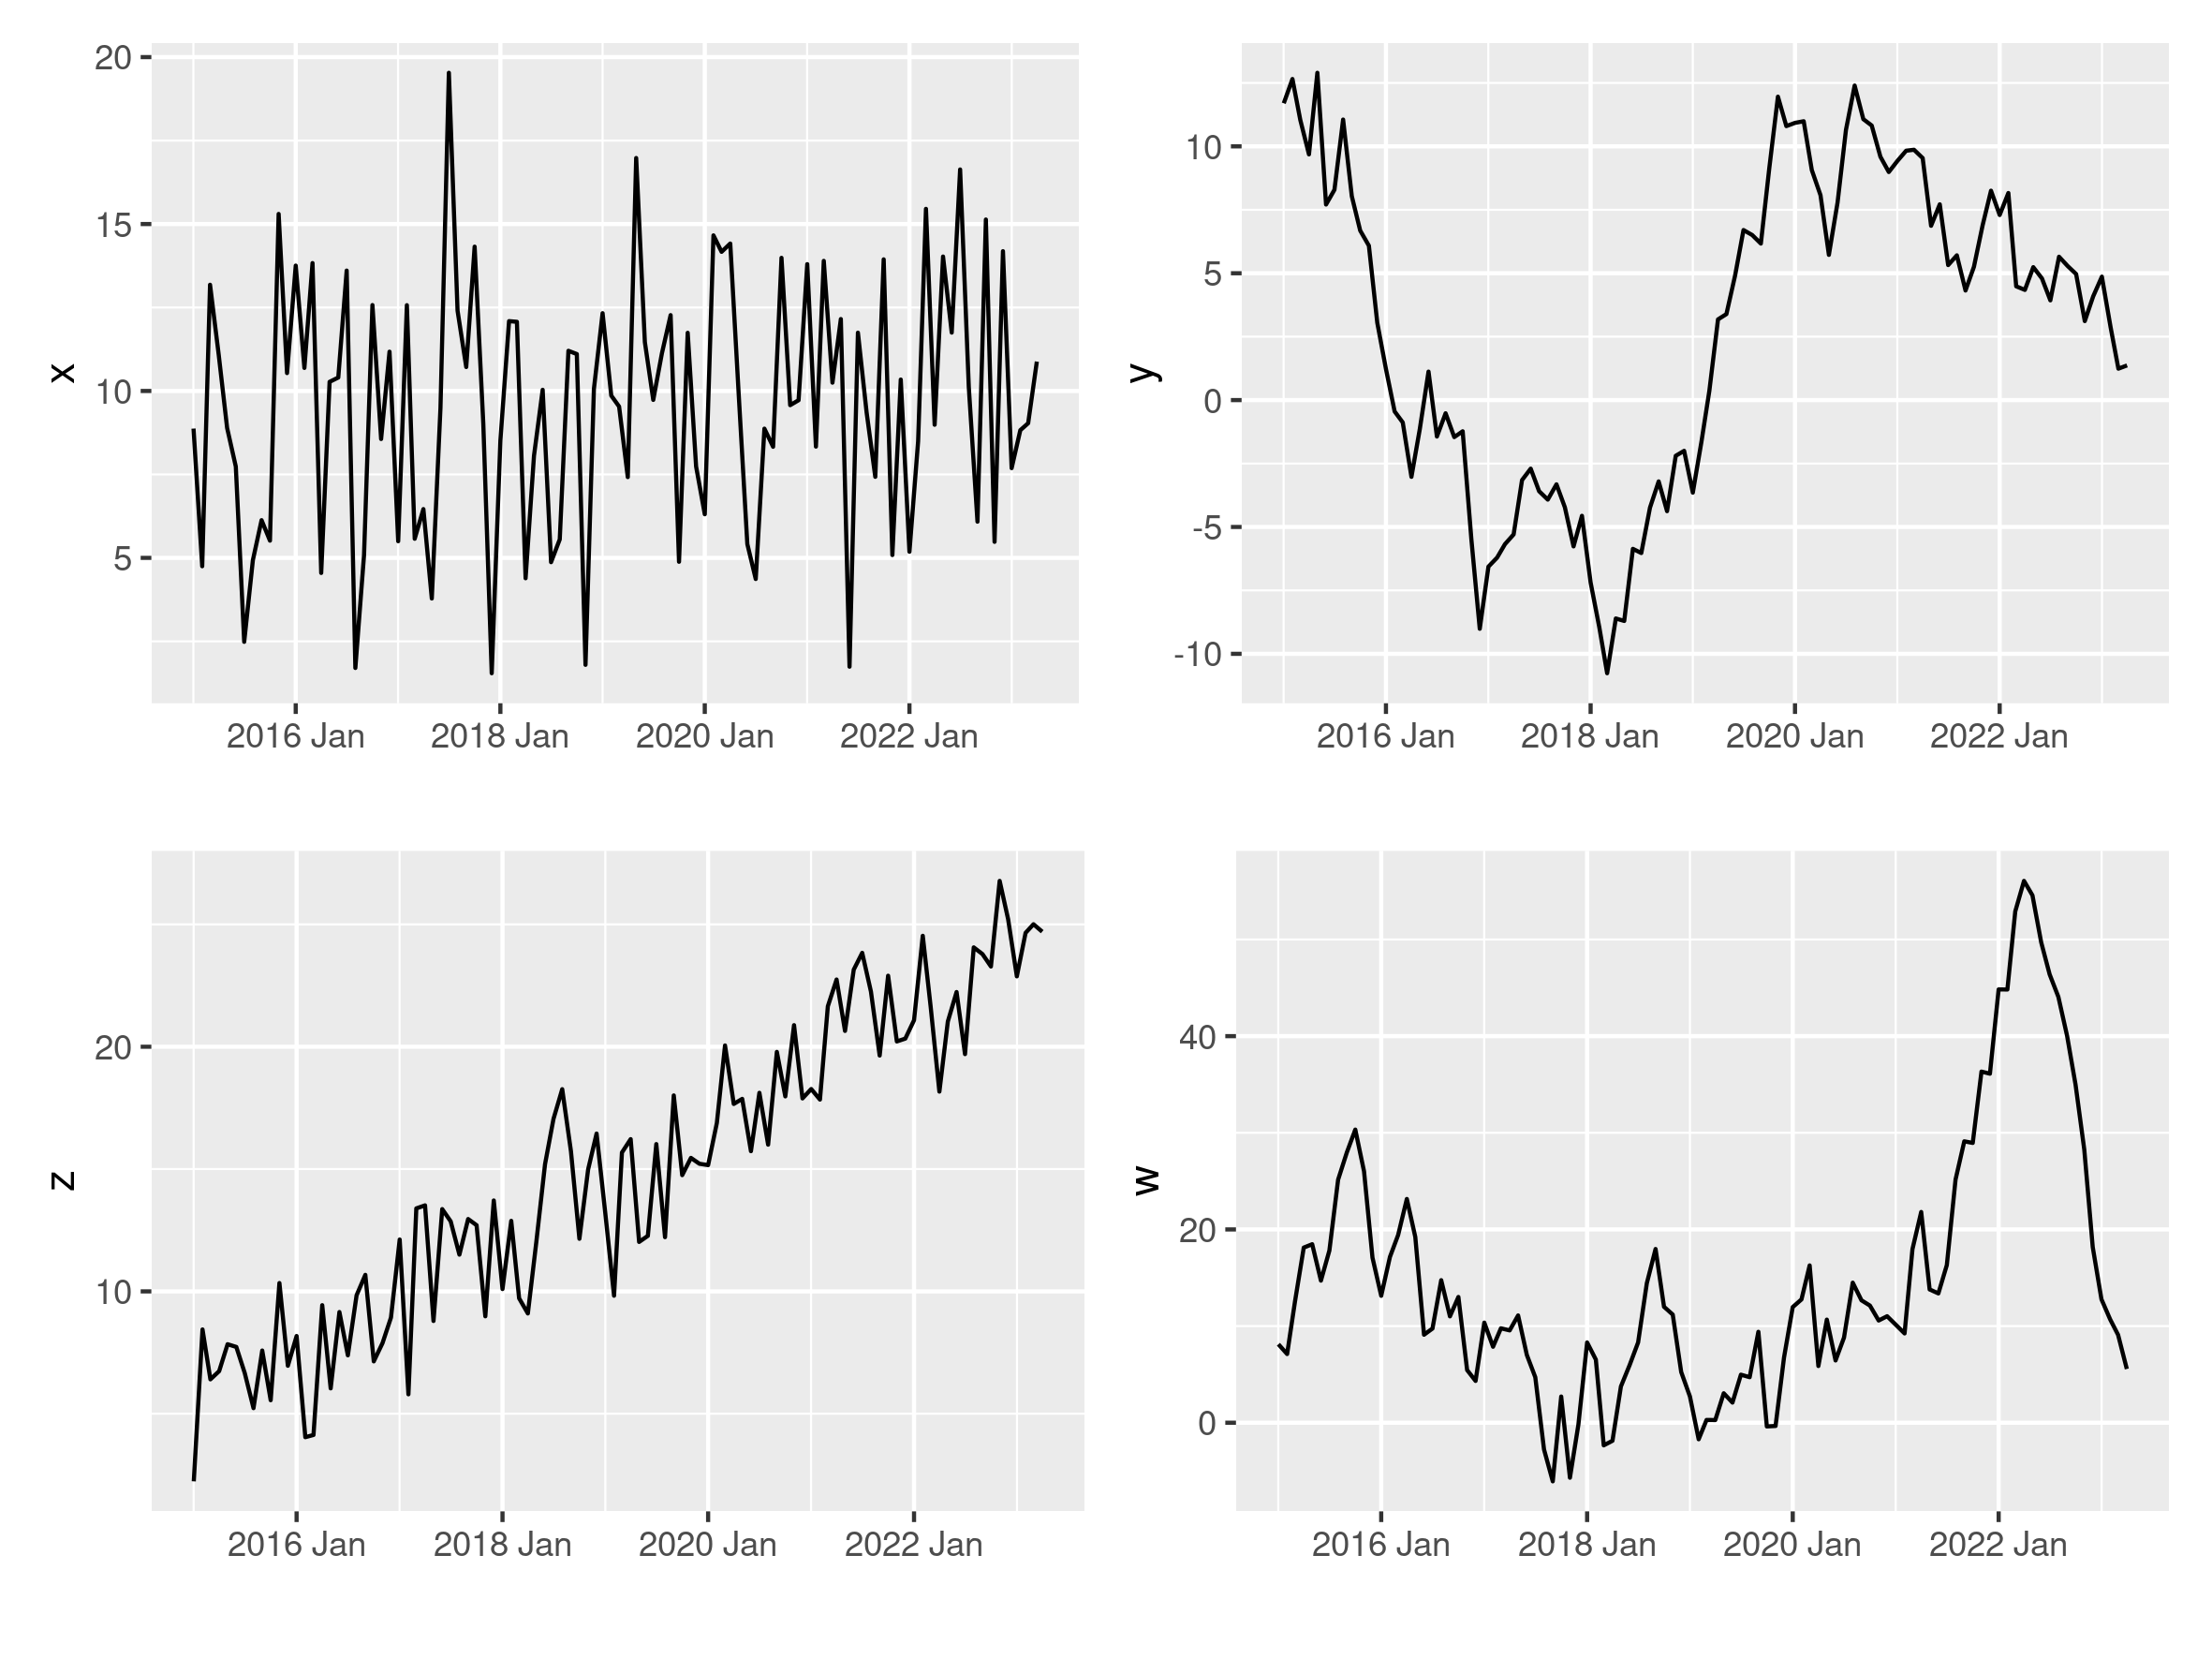
\includegraphics[width=\textwidth]{pictures/om_ts_06-027.png}
\end{frame}


\begin{frame}{ARIMA: Summary}
	
	\begin{itemize}[<+->]
		\item $ARMA$ is for \alert{stationary} series
		\item Sometimes $\Delta y_t$ or $\Delta^2 y_t$ is stationary
		\item Choose between $ARMA$ and $ARIMA$
	\end{itemize}
\end{frame}


\begin{frame} % название фрагмента
	
	\videotitle{SARIMA process}
	
\end{frame}



\begin{frame}{SARIMA process: Plan}
	\begin{itemize}[<+->]
		\item Seasonal $ARMA$

		\item Seasonal $ARIMA$
		
		\item Choosing between models
	\end{itemize}
	
\end{frame}


\begin{frame}
	\frametitle{Seasonality and $ARIMA$}
	
	Using $ARMA$ and $ARIMA$ models, we can model seasonality!
	
	\pause
	\[
	MA(12): y_t = c + u_t + a_1 u_{t-1} + a_2 u_{t-2} + \ldots + a_{12} u_{t-12}.
	\]
	\[
	ARIMA(12, 1, 0): \Delta y_t = c + u_t + b_1 \Delta y_{t-1} + \ldots + b_{12} \Delta y_{t-12}.
	\]
	
\end{frame}



\begin{frame}
	\frametitle{ARMA should be economical!}
	
	Let's focus on \alert{non-zero} coefficients!
	\pause
	\begin{block}{Definition}
		If the stationary $ARMA$ model for $y_t$ can be written with fewer parameters as
		\[
		P_{non}(L)P_{seas}(L^{12}) y_t = c + Q_{non}(L) Q_{seas}(L^{12}) u_t,
		\]
		where the degrees of the lag polynomials are $\deg P_{non} =p$, $\deg P_{seas} =P$, $\deg Q_{non} =q$, $\deg Q_{seas} =Q$,
		then it is also called $SARMA(p, q)(P, Q)[12]$
	\end{block}
\end{frame}


\begin{frame}
	\frametitle{Examples}
	
	\begin{itemize}
		\item $SARMA(\alert{1},0)(0,\alert{2})[12]$
	\end{itemize}
	
	
		\[
		(1 - b_{\alert{1}} L) y_t = c + (1 + d_1 L^{12} + d_{\alert{2}} L^{24}) u_t;
		\]
	
	\pause 
		
	\begin{itemize}
		
		\item $SARMA(0,\alert{2})(\alert{1},0)[12]$
	\end{itemize}		

		\[
(1 - f_{\alert{1}} L^{12}) y_t = c + (1 + a_1 L + a_{\alert{2}} L^2) u_t;
\]

		
	\pause 
		
	\begin{itemize}
		
		\item $SARMA(\alert{1},\alert{2})(2,1)[12]$
	\end{itemize}



		\[
		(1 - f_1 L^{12} - f_{\alert{2}} L^{24}) (1 - b_{\alert{1}} L^1) y_t = c + (1 + a_1 L + a_2 L^2) (1 + d_1 L^{12}) u_t
		\]
	
	
	
\end{frame}





\begin{frame}
	\frametitle{SARIMA}
	
	By analogy with the difference $\Delta y_t = y_t - y_{t-1}$, we can consider the seasonal difference $\Delta_{12} y_t = y_t - y_{t-12}$
	
	\pause
	\begin{block}{Definition}
		If the series $z_t = \Delta^{\alert{d}} \Delta^{\alert{D}}_{12} y_t$ is described by the stationary model $SARMA(p, q)(P, Q)[12]$ ,
		then $y_t$ is said to be described by the $SARIMA(p, \alert{d}, q)(P, \alert{D}, Q)[12]$ model
	\end{block}
	\pause
	$d$ is the number of times the first difference should be taken $\Delta = 1 - L$;
	
	$D$ is the number of times the seasonal  difference should be taken $\Delta_{12} = 1- L^{12}$;
	\pause
	$y_t \sim SARIMA(0, 0, 2)(1, \alert{1}, 2)[12]$ means that
	
	$\Delta_{12} y_t \sim SARMA(0, 2)(1, 2)[12]$
\end{frame}

\begin{frame}
	\frametitle{How to choose?}
	
	$SARIMA(p, 0, q)(P, 0, Q)$ or $SARIMA(p, 0, q)(P, 1, Q)[12]$?
	
	\begin{itemize}
		\onslide<2->{\item Analyse the \alert{graph}!}
				
		\onslide<3->{\item Evaluate all these models and choose the best one by \alert{cross-validation}}
		\onslide<4->{Time consuming!}
		
		\onslide<5->{\item \alert{You cannot use $AIC$}!}
		\onslide<6->{The conditional and unconditional likelihood functions contain different numbers of terms.}
		
		\onslide<7->{\item There are \alert{unit root tests}!}
		
		\onslide<8->{And rules of thumb\ldots}
	\end{itemize}
	
\end{frame}


\begin{frame}
	\frametitle{STL decomposition and the power of seasonality}
	
	\onslide<1->{Step 1. Find the $STL$ expansion of the series $(y_t)$
		\[
		y_t = trend_t + seas_t + remainder_t
		\]}
	
	\onslide<2->{Step 2. Calculate the strength of seasonality
		\[
		F_{seas} = \max\left\{1 - \frac{\sVar(remainder)}{\sVar(seas + remainder)}, 0 \right\}
		\]}
	
	\onslide<3->{Step 3. If the strength of seasonality is above the threshold, then move to $\Delta_{12} y_t = y_t - y_{t-12}$}
	
\end{frame}



\begin{frame}{SARIMA: Summary}
	
	\begin{itemize}[<+->]
		\item Seasonal ARIMA is more compact
		\item The strength of seasonality from the \alert{STL} expansion is used to decide if a seasonal difference $\Delta_{12} y_t$ is needed

	\end{itemize}
\end{frame}

